\section{Renewal Reward Theorem and load}
\label{sec:renew-reward-theor}

\opt{solutionfiles}{
\subsection*{Theory and Exercises}
\Opensolutionfile{hint}
\Opensolutionfile{ans}
}


We start with stating and proving (graphically) the \recall{renewal reward theorem}.
In the sequel we will see many applications of this theorem.
In this section we use it to relate the fraction of time the server is busy in a $G/G/1$ queue to the job arrival rate and the expected job service time.


The renewal reward theorem is very useful, and states intuitively that when customers arrive at rate $\lambda$ and each customer pays an average amount $X$, then the system earns money at rate $Y=\lambda X$.
\Cref{fig:renewal} provides graphical motivation about why this theorem is true; \citet{el-taha98:_sampl_path_analy_queuein_system} gives a (simple) proof.

\begin{theorem}[Renewal Reward Theorem, $Y=\lambda X$]
  Consider epochs $\{T_k, k=0, 1, \ldots\}$ such that  $0=T_0 < T_1 < \cdots$
  Let $N=\{N(t), t\geq 0\}$ be the associated counting process with $N(t) = \max\{k : T_k \leq t\}$.
  Let $\{Y(t), t\geq 0\}$ be a non-decreasing right-continuous (deterministic) process.
  Define $X_k = Y(T_k)-Y(T_{k-1})$.
  Suppose that $N(t)/t\to\lambda$ as $t\to\infty$, where $0<\lambda < \infty$.
  Then $Y(t)/t$ has a limit iff $n^{-1}\sum_k^n X_k$ has a limit, and then $Y=\lambda X$. In other words, 
 \begin{equation*}
   \lim_{t \to \infty} \frac{Y(t)}t=Y \iff \lim_{n \to \infty} \frac 1n\sum_{k=1}^n X_k = X, 
 \end{equation*}
and then $Y=\lambda X$. 
\end{theorem}


\begin{figure}[ht]
  \centering
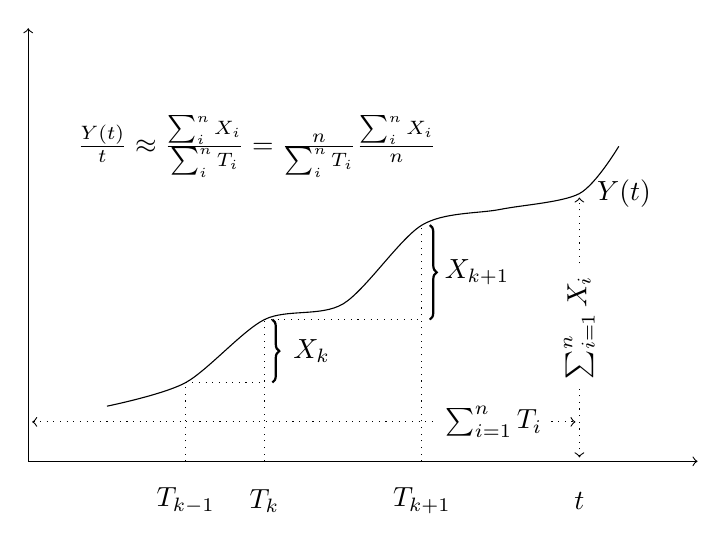
\begin{tikzpicture}[scale=1]
%axis
\draw[->] (0,0) -- coordinate (x axis mid) (8.5,0);
\draw[->] (0,0) -- coordinate (y axis mid) (0,5.5);
%\node[below=0.2cm] at (x axis mid) {$t$};

\draw plot [smooth] coordinates {(1,0.7) (2,1) (3,1.8) (4,2) (5,3) (6,3.2) (7, 3.4) (7.5,4.0)};
\node[right]  at (7.1,3.4) {$Y(t)$};
\node  at (7.,-0.5) {$t$};

\node  at (2.,-0.5) {$T_{k-1}$};
\draw[dotted] (2,0)--(2,1);
\draw[dotted] (2,1)--(3,1);


\node  at (3.,-0.5) {$T_{k}$};
\draw[dotted] (3,0)--(3,1.8);
\draw[dotted] (3,1.8)--(5,1.8);

\draw [
    thick,
    decoration={brace, mirror, raise=0.1cm },
    decorate
] (3,1) -- (3,1.8)
node[pos=0.5, xshift=0.6cm]  {$X_k$}; 


\node  at (5.,-0.5) {$T_{k+1}$};
\draw[dotted] (5,0)--(5,3);

\draw [
    thick,
    decoration={brace, mirror, raise=0.1cm },
    decorate
] (5,1.8) -- (5,3)
node[pos=0.5, xshift=0.7cm]  {$X_{k+1}$}; 

\node[right] at (0.5,4) {$\frac{Y(t)}t \approx \frac{\sum_i^n X_i}{\sum_{i}^n T_i} = \frac{n}{\sum_{i}^n T_i} \frac{\sum_i^n X_i}n $};


\draw[dotted,<->, =stealth] (7,0.05)--(7,3.35) node[midway, rotate=90, fill=white] {$\sum_{i=1}^n X_i$};
\draw[dotted,<->, =stealth] (0.05,0.5)--(6.95,0.5) node[pos=0.85, fill=white] {$\sum_{i=1}^n T_i$};
\end{tikzpicture}
\caption{A graphical `proof' of $Y=\lambda X$. Here $Y(t)/t\to Y$, $n/\sum^n_i T_i\to \lambda$ and $n^{-1}\sum_i^n X_i \to X$.  (Observe that in the
  figure $X_k$ does not represent an inter-arrival time; instead it
  corresponds to the increment of (the graph of) $Y(t)$ between two
  consecutive epochs $T_{k-1}$ and $T_k$ at which $Y(t)$ is
  observed.) }
  \label{fig:renewal}
\end{figure}

Define the \recall{load} or \recall{utilization} as the limiting fraction of time the server is busy, i.e.,
\begin{equation*}
  \rho = \lim_{t\to\infty} \frac 1 t \int_0^t \1{L(s)>0} \d s.
\end{equation*}

\begin{exercise}
Use the renewal reward theorem to prove that $\rho = \lambda \E S$.
\begin{hint}
  Define $Y(t) = \int_0^t \1{L(s)>0} \d s$ as the total amount of time the server has been busy up to the time $t$.
  Then take as epochs $T_k = D_k$ and use rate stability.
\end{hint}
\begin{solution}
  It is evident that $X_k =  Y(D_k)-Y(D_{k-1})=S_k$, hence $X = \lim_{n\to\infty} n^{-1}\sum_{k=1}^n X_k = \E S$.
  Also $\lim_{t\to\infty} Y(t)/t=\rho$.
  Finally, in the relation $Y = \lambda X$, the $\lambda$ is $\delta$ since we consider departure epochs $T_k = D_k$, rather than $A_k$.
  By the renewal reward theorem $Y=\lambda X$ we get that $\rho = \delta \E S$.
  Finally, by rate-stability, the job arrival rate $\lambda = \delta$, hence $\rho = \lambda \E S$.
\end{solution}
\end{exercise}


\begin{exercise}
  We can derive the relation $\rho = \lambda \E S$ in a somewhat more direct way by considering the fact that
\begin{equation*}
  \sum_{k=1}^{A(t)} S_k \geq \int_0^t \1{L(s)>0} \d s \geq   \sum_{k=1}^{D(t)} S_k.
\end{equation*}
Explain this, and complete the argument.
\begin{solution}
Observe that
since $t$ can lie half way a service interval and $A(t) \geq D(t)$. As
$A(t)\to \infty$ as $t\to\infty$,
\begin{equation*}
  \lim_{t\to\infty} \frac 1 t\sum_{k=1}^{A(t)} S_k = 
  \lim_{t\to\infty} \frac{A(t)}t \frac{1}{A(t)} \sum_{k=1}^{A(t)} S_k = 
  \lim_{t\to\infty} \frac{A(t)}t \cdot \lim_{t\to\infty}\frac{1}{A(t)} \sum_{k=1}^{A(t)} S_k = \lambda \E S.
\end{equation*}
Applying similar limits to the other inequality gives
\begin{equation*}
\lambda \E S \geq \rho \geq \delta \E S.
\end{equation*}
Hence, if $\delta=\lambda$, $\rho = \lambda \E S$.  

Note that this is in fact the same argument as that underlies the renewal reward theorem. Henceforth we will just use the renewal reward theorem. 
\end{solution}
\end{exercise}


From the identities $\lambda^{-1} = \E X$ and $\mu^{-1} = \E S$, we get
a further set of relations:
\begin{equation*}
  \rho = \lambda \E S = \frac{\lambda}{\mu} = \frac{\E S}{\E X}.
\end{equation*}
Thus, the load has also the interpretation as the rate at which jobs
arrive times the average amount of work per job.  Finally,
recall that for a system to be rate-stable, it is necessary that
$\mu> \lambda$, implying in turn that $\rho < 1$. The relation
$\rho=\E S/ \E X < 1$ then tells us that the average time it takes to
serve a job must be less than the average time between two consecutive
arrivals, i.e., $\E S < \E X$. In fact, when $\mu < \lambda$, it is easy to check with simulation that the queue length
grows roughly linearly with slope $\lambda - \mu$.


\begin{exercise}
  Consider a queueing system with $c$ servers with identical production rates $\mu$.
  What would be a reasonable stability criterion for this system?
  \begin{hint}
What is the rate in, and what is the service capacity?
  \end{hint}
  \begin{solution}
    The criterion is that $c$ must be such that $\lambda < c\mu$.
    (Thus, we interpret the number of servers as a \emph{control}, i.e., a `thing' we can change, while we assume that $\lambda$ and $\mu$ cannot be easily changed.)
    To see this, we can take two different points of view.
    Imagine that the $c$ servers are replaced by one server that works $c$ times as fast.
    The service capacity of these two systems (i.e., the system with $c$ servers and the system with one fast server) is the same, i.e., $c\mu$, where $\mu$ is the rate of one server.
    For the system with the fast server the load is defined as $\rho =\lambda/c\mu$, and for stability we require $\rho<1$.
    Another way to see it is to assume that the stream of jobs is split into $c$ smaller streams, each with arrival rate $\lambda/c$.
    In this case, applying the condition that $(\lambda/c )/\mu<1$ per server leads to the same condition that $\lambda/(c\mu) < 1$.
  \end{solution}
\end{exercise}



\opt{solutionfiles}{
\Closesolutionfile{hint}
\Closesolutionfile{ans}
\subsection*{Hints}
\input{hint}
\subsection*{Solutions}
\input{ans}
}
%\clearpage


%%% Local Variables:
%%% mode: latex
%%% TeX-master: "../companion"
%%% End:
